To start off, we have to talk about what becomes of a star during a Type - IIp supernova.
When the star explodes, an envelope of gas expands in all directions at a high rate of speed.
The speed of the expanding gas can be determined by looking at the spectrum of the light being 
emitted by the gas and comparing it to another source to see how blueshifted it is. This is done 
using spectroscopy. 
\\
For the Expanding Photosphere Method to work, we have to assume that the expanding photosphere of gas 
is thin and uniform, meaning that it expands evenly in all directions away from the star.
\\
The equation we will use to determine the distance is called the angular radius.
\\
\begin{figure} [h!]
    \begin{center}
    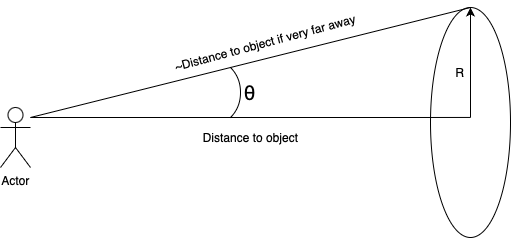
\includegraphics[width=0.5\textwidth]{Angular_Radius.png}
    \end{center}
    \label{fig:angular_radius}
    \caption{A diagram of angular radius.}    
\end{figure}
\\
In the above figure \ref{fig:angular_radius} there is a disk, a person, and a right triangle between them.
Lets assume for the sake of explination that the disk is the Sun and the person is on Earth.
The distance between the person and the Sun is $d$ and the radius of the Sun is $R$.
The angle $\theta$ created by the right triangle formed is called the angular radius. 
We can write this relationship as:
\\
\begin{equation}\label{initial}
    \tan{\theta} = \frac{\textrm{R}}{\textrm{d}}
\end{equation}
\\
The next thing we must take into account is the fact that the supernova that we are looking at is incredibly far away.
This means the angular radius $\theta$ approaches 0. Using the small angle approximation, $\tan{\theta}$ becomes $\theta$, 
and the equation \ref{initial} becomes:
\\
\begin{equation}\label{eqn:after_saa}
    \theta = \frac{\textrm{R}}{\textrm{d}}
\end{equation}
\\
Because the photosphere is expanding, the radius $R$ is increasing over time with a measurable velocity. This allows us to set R to:
\\
\begin{equation}\label{eqn:radius}
    R = v(t-t_0)
\end{equation}
\\
Where $v$ is the velocity of the photosphere at that time, $t$ is the time since explosion, and $t_0$ is the time of explosion.
\\
Next, since the supernova is very far away, we have to account for time dialation. This can be accomplished by using a constant in the following way:
\\
\begin{equation}\label{eqn:distance}
    d = d(1+z)
\end{equation}
\\
Where $d$ is the distance to the supernova and $z$ is the time dialation constant.
\\
This gives us:
\\
\begin{equation}\label{eqn:pre_linear}
    \theta = \frac{v(t-t_0)}{d(1+z)}
\end{equation}
\\
We rearrange this equation to get it into slope intercept form:
\\
\begin{equation}\label{eqn:slope_incercept}
    t = \frac{\theta}{v}(1+z)d + t_0
\end{equation}
\\
Where $(1+z)d$ is the slope and $t_0$ is the intercept. With this function \ref{eqn:slope_incercept} 
we can graph data points (in $(\frac{\theta}{v}, t)$ form) and find the line of best fit to determine the distance.
The graphed data will look like figure \ref{fig:distance_graph}.
\\
\begin{figure} [h!]
    \begin{center}
    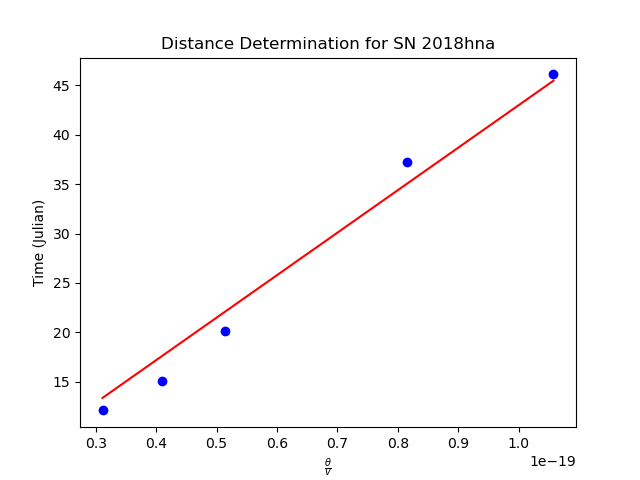
\includegraphics[width=0.5\textwidth]{Distance_Graph.png}
    \end{center}
    \label{fig:distance_graph}
    \caption{The graph of data points in blue and line of best fit in red.}    
\end{figure}
\\
Depending on the method of determining the angular radius $\theta$, you may have to make multiple distances 
like figure \ref{fig:distance_graph}. I will speak more about this in the data section.




